\documentclass[11pt, letterpaper]{article}		% The percent symbol in your code starts a comment.  The comment ends at the next linebreak.

\usepackage[english]{babel} 		% Packages add functionality and style conventions to your documents. Don't edit this section!
\usepackage[utf8]{inputenc}			% Necessary for character encoding
\usepackage{geometry}
\usepackage{amsmath, amssymb,amsthm}% Required math packages
\usepackage{graphicx}				% For handling graphics
\usepackage{hyperref}				% For clickable links in the final PDF
\usepackage{minted} %Pacakge for long blacks of code
\usepackage{verbatim} %Package for in-line code
\usepackage{graphicx} %package to manage images
\graphicspath{ {images/} }
\usepackage{listings}

\theoremstyle{definition}
\newtheorem{theorem}{Theorem}
\newtheorem{lemma}[theorem]{Lemma}
\newtheorem{prop}[theorem]{Proposition}
\newtheorem{claim}[theorem]{Claim}

\setlength{\topmargin}{0pt}
\setlength{\headsep}{0pt}
\textheight = 600pt

\newcommand{\ds}{\displaystyle}
\newcommand{\postcode}{\vspace{-3ex}\text{}\\}
\renewcommand\labelitemii{$\rightarrow$}
\renewcommand\labelitemiii{$\square$}

\title{Solving Nerdle with Entropy}
\author{Joseph Wu }
\date{}

\begin{document}
\maketitle
\medskip
\hrule
\medskip

\section{Introduction}
During Wordle's initial burst of popularity, the game inspired a slew of clones, all of which kept Wordle's core \textit{ethos} of ``guess the secret thing while the game gives you hints''. One of these games was Nerdle, an arithmetic-based Nerdle clone where instead of trying to guess a 5-letter word, you would try to guess an 8-character arithmetic equation.
\begin{figure}[H]
    \centering
    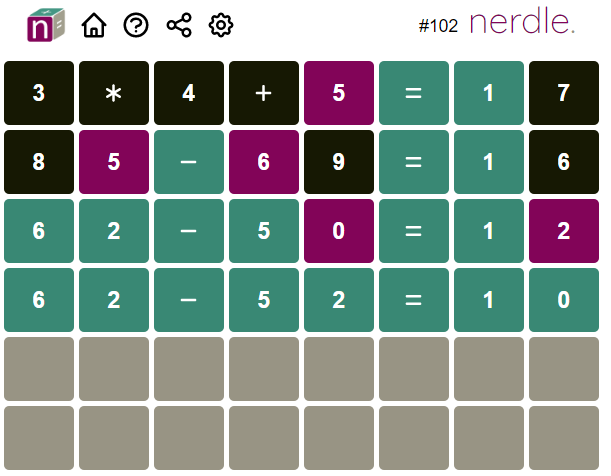
\includegraphics[width=10cm]{nerdle_game.png}
    \caption{A game of Nerdle, played to completion.}
\end{figure}


In February, YouTube math educator 3Blue1Brown released a video entitled ``Solving Wordle using information theory'' where he discusses using the idea of entropy to develop an efficient Wordle-solving algorithm. Games like Wordle do indeed tickle the fancy of 

It is a relatively simple game, making it easy to abstract into code and math, while still having enough complexity to be interesting and worthwile of play.
\section{Wordle}

On their surface, Wordle and Nerdle seem to be quite similar: try to find a secret phrase by making guesses while the game tells you how much those guesses differ from the actual solution. What differentiated Wordle and Nerdle are what actually qualifies as a ``phrase''. Here it is useful to introduce the terms \textbf{guess space} and a \textbf{solution space}. The \textbf{solution space} is the list of all phrases that might potentially be a secret phrase. The \textbf{guess space} is the list of all valid guesses (i.e. guesses that the game will accept). It makes sense that the solution space is a subset of the guess space: all potential answers are valid guesses but not all guesses are potential answers. Consider, for example, the word \texttt{ACKEE}. It is a perfectly-valid English word (it's a west African fruit related to the lychee, for the curious) that the Wordle game will happily accept as a valid guess; however, due to the word's obscurity, we will never have to suffer through a puzzle where \texttt{ACKEE} is the word-of-the-day.


\section{Finding the Guess Space}
In order to generate phrase-of-the-days and check guesses, Wordle maintains a list of all valid words. Nerdle, however, uses a parser that checks 


\end{document}